\documentclass{revtex4-2}
\usepackage{graphicx} % Required for inserting images

\usepackage{physics}

\begin{document}

\title{test for latexdiff}
\author{Ivan Toftul}
\date{May 2023}

\maketitle

\section{First section}

This is a revision
\begin{equation}
    \int \dd \Omega Y_{\ell m} (\vartheta, \varphi) Y_{\ell^{\prime} m^{\prime}} (\vartheta, \varphi) = \delta_{\ell \ell^{\prime}} \delta_{m m^{\prime}}
\end{equation}
It is not discussed here~\cite{Toftul2019Oct}. Fig.~\ref{fig:figure1} is cool.

\begin{figure}
    \centering
    %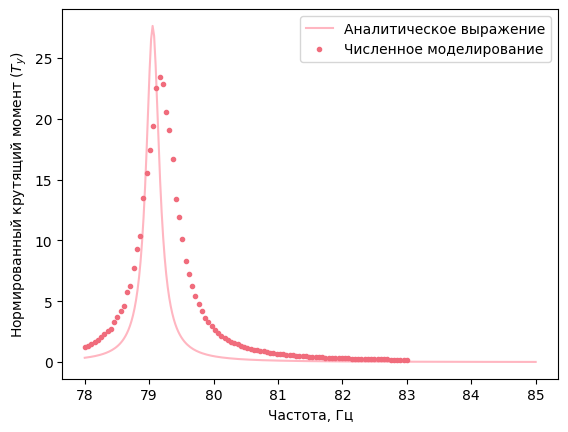
\includegraphics[width=0.7\linewidth]{fig/figure1.png}
    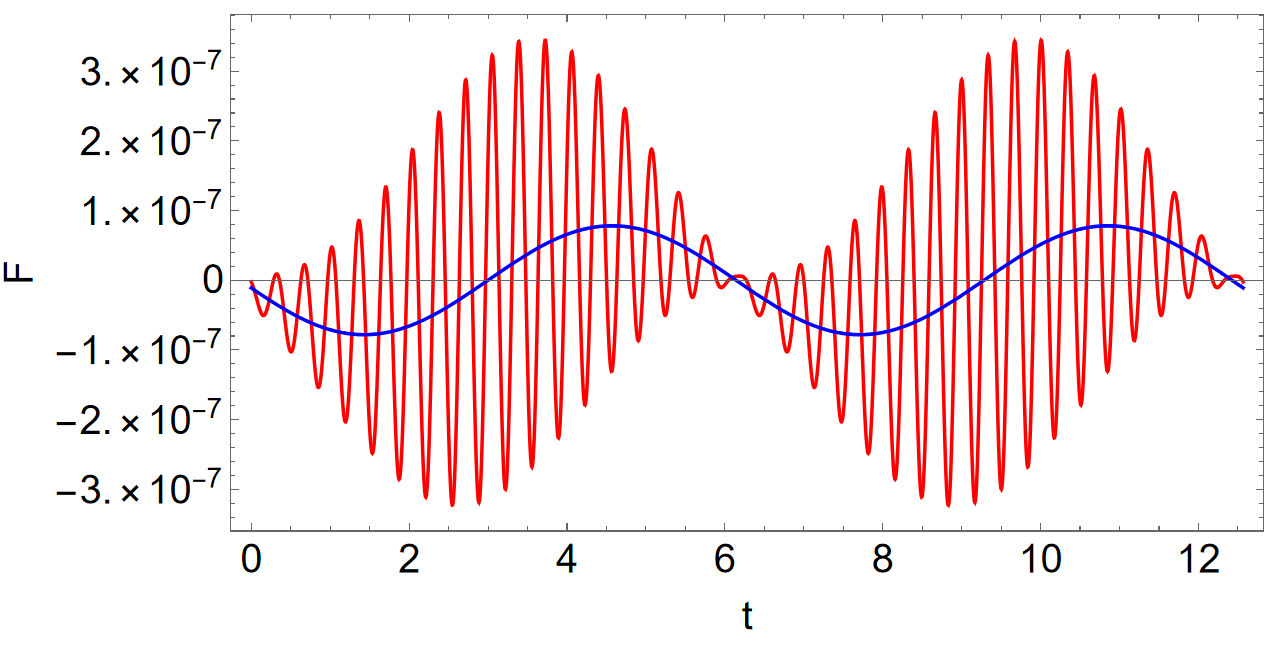
\includegraphics[width=0.7\linewidth]{fig/image.png}
    \caption{This is the first figure.}
    \label{fig:figure1}
\end{figure}

\section{Second section}

Wow! Look at this
\begin{equation}
    \begin{bmatrix}
\tensor{\alpha}_{\text{ee}} & \tensor{\alpha}_{\text{em}} \\
\tensor{\alpha}_{\text{me}} & \tensor{\alpha}_{\text{mm}} 
\end{bmatrix} / \begin{bmatrix}
\alpha_{pp} & \vec{\alpha}_{pv} \\
\vec{\alpha}_{vp} & \tensor{\alpha}_{vv} 
\end{bmatrix}
\end{equation}

\begin{figure}
    \centering
    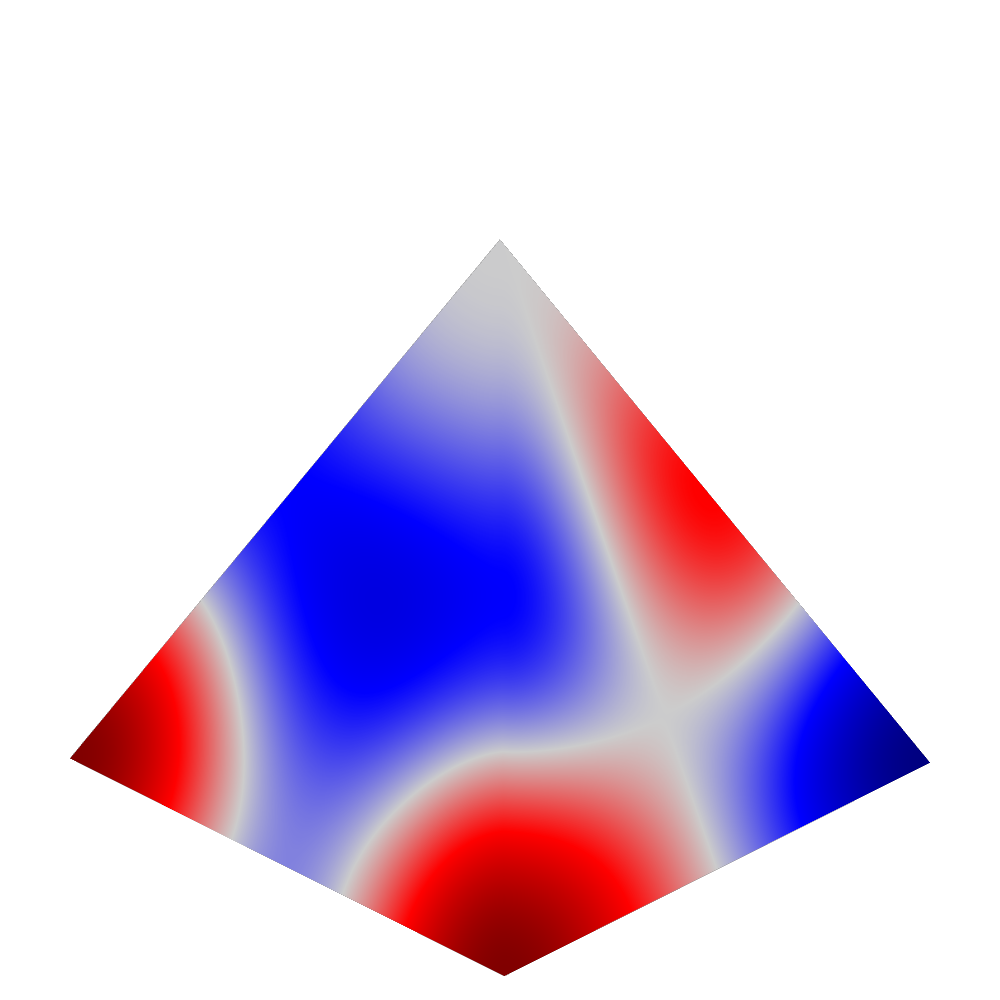
\includegraphics[width=0.3\linewidth]{fig/E_2_2.png}
    \caption{This is a mode distribution.}
    \label{fig:mode}
\end{figure}

\bibliography{refs}

\end{document}
